\documentclass[12pt]{article}
\usepackage{amsmath}
\usepackage{mathtools}
\usepackage{epigraph}
\usepackage{cancel}
\usepackage{xcolor}
\newcommand\Ccancel[2][black]{\renewcommand\CancelColor{\color{#1}}\cancel{#2}}
\addtolength{\oddsidemargin}{-1.25in}
\addtolength{\evensidemargin}{+1.25in}
\addtolength{\textwidth}{1.75in}

\addtolength{\topmargin}{-.875in}
\addtolength{\textheight}{1.75in}

\begin{document}

\begin{titlepage}
\title{
SWIRL Documentation}


\author{ Jeffrey Severino
 \\
University of Toledo \\
Toledo, OH  43606 \\
email: jseveri@rockets.utoledo.edu  }

\maketitle

\end{titlepage}
\tableofcontents
\newpage
\section{Divergence operations in new coordinate systems}

%\epigraph{The introduction of numbers as \textit{coordinates} is an act of violence."} {\textit{Hermann Weyl}}

%Hermann Weyl was a renown mathematician and physicist who has made revolutionary contributions to the field of differential geometry and topology. In his work on manifolds, he proposed the idea of working without coordinates and showed the application of multi-variable without the need to define a coordinate system , using coordinates when only absolutely necessary. This perspective emphasizes the distinction between quantities and the various coordinates systems that can be used to describe their change and behavior.
The divergence, ($\nabla$), represents the operation of taking derivatives of a vector field. However, understanding the mathematical and physical representation of the divergence operator into new coordinate systems serves as a good prerequisite for the application of the Navier Stokes equations for the evaluation of aerodynamic models in unusual flow domains. Although there are many resources that will provide equations in varying coordinate systems, the derivation offers insight into the advantages and drawbacks of using a new reference frame for a flow domain. The divergence operator in Cartesian coordinates is,
%This is also important because eigenmode analysis tells us the domain of a pulse traveling through the domain at a frequency that is intrinsic to the flow itself



\begin{align*}
\vec{\nabla} \equiv
\hat{e}_x \frac{\partial }{\partial x}  %...
+ \hat{e}_y \frac{\partial }{\partial y}  %...
	+ \hat{e}_z \frac{\partial }{\partial z}                      = 0
\label{Divergence_Operator}
\end{align*}

The vectors, $\hat{e}_x,\hat{e}_y,\hat{e}_z$ (commonly denoted in literature as $\hat{i}$,$\hat{j}$,$\hat{k}$) are the basis vectors of the Cartesian coordinate system. The vector hat ( $\vec{}$ ) reminds us that divergence operation includes a scalar product of  the basis vectors and the individual derivative terms themselves.
These basis vectors \textit{scale} with the derivatives $d/dx$ $d/dy$ $d/dz$ in the direction of these basis vectors themselves. This implicitly captures the coordinate system and assumptions that corresponds to the basis vectors themselves.

To relate the basis vectors of the cylindrical coordinate system to the Cartesian coordinate system, we use the following relations,
\begin{align*}
	r 
	&= \sqrt{x^2 + y^2} \\
	\theta 
	&= \tan^{-1} \Big( \frac{y}{x} \Big) \\
	&= \cos^{-1} \Big( \frac{x}{r} \Big) \\
	&=\sin^{-1} \Big( \frac{y}{r} \Big)		
\end{align*}
	Note that the equation above also establishes $x   = r\cos \theta$ and $y = r\sin\theta$. The Cartesian basis vectors are related to the cylindrical basis vectors of the new coordinate system by,

\begin{align*}
	\hat{e}_r 
	&= \hat{e}_x \cos \theta + \hat{e}_y \sin \theta \\
	\hat{e}_{\theta} 
	&= -\hat{e}_x \sin \theta + \hat{e}_y \cos \theta \\
	\hat{e}_z 	 
	&= \hat{e}_z %\label{eq:cylindrical_basis_vectors}
\end{align*}

Defining these relationships, (they'll be useful later)

\begin{align*}
	\frac{\partial \hat{e}_{r	  }}{\partial r} 
	&= \frac{\partial \hat{e}_{\theta}}{\partial r} 
	= \frac{\partial \hat{e}_{z}	   }{\partial r} = 0 \\
	\frac{\partial \hat{e}_{r	  }}{\partial \theta} 
	&=	-\hat{e}_x \sin \theta + \hat{e}_y \cos \theta                = \hat{e}_{\theta}\\
	\frac{\partial \hat{e}_{\theta	  }}{\partial \theta}
	&= -\left(
	\hat{e}_x \cos \theta + \hat{e}_y \sin \theta
	\right) = 
	-\hat{e}_{r}
\end{align*}

The multi-variable chain rule for differentiation is then used to express the Cartesian variables, $\frac{\partial}{\partial x}$,$\frac{\partial}{\partial y}$,$\frac{\partial}{\partial z}$ , with respect to the cylindrical variable.

\begin{align*}
	\frac{\partial }{\partial x}
	&= \frac{\partial }{\partial r}\frac{d r}{d x} +
	\frac{\partial }{\partial \theta}\frac{d \theta}{d x} +
	\frac{\partial }{\partial z}\frac{d z}{d x} 
	%\label{ddx}
\end{align*}

\begin{align*}
	\frac{\partial }{\partial y}
	&=
	\frac{\partial }{\partial r} 	 \frac{d r}{d y} +
	\frac{\partial }{\partial \theta} \frac{d \theta}{d y} + \frac{\partial }{\partial z}     \frac{d z}{d y}
%\label{ddy}
\end{align*}


By,finding the derivatives of $r$ $\&$ $\theta$ with respect to $x$ and $y$, we can substitute terms in the Cartesian divergence definition. First, $\frac{dr}{dx}$ \& $\frac{dr}{dy}$ is calculated,

% dr/dx
\begin{align*}
 	\frac{dr}{dx}                                      
	&= \frac{d}{dx} \Bigg(\Big[ x^2 + y^2 \Big]^{1/2}\Bigg) \\
	&= \frac{1}{2} \Big[ x^2 + y^2 \Big]^{-1/2} (2x) \\
 	&=	\frac{x}{\sqrt{x^2+y^2}}\\
 	&= \frac{r cos\theta}{r}\\
 	& \boxed{\frac{dr}{dx} = cos\theta} 
\end{align*}
% dr/dy
\begin{align*}
	\frac{dr}{d y}
	&= \frac{d}{dy} \Bigg(\Big[ x^2 + y^2 \Big]^{1/2}\Bigg) \\
	&= \frac{1}{2}\Big[x^2 + y^2\Big]^{-1/2}(2y) \\
	&= \frac{y}{\sqrt{x^2+y^2}} \\
	&= \frac{r sin\theta}{r}\\
	& \boxed{\frac{dr}{d y} = sin\theta} 
\end{align*}
%d\theta/dx
Then, $\frac{d\theta}{dx}$ \& $\frac{d\theta}{dy}$ is found.
\begin{align*}
	\frac{d \theta}{d x} 
	&= \frac{d}{dx} \Bigg(tan^{-1} \Big(\frac{y}{x}\Big)\Bigg)  \\
	&= \frac{d}{du}tan^{-1}(u) \frac{d}{dx} \Big( \frac{y}{x} \Big)\\
	&= \frac{1}{u^2  + 1} \frac{-y}{x^2} \\
	&= -\frac{y}{y^2 + x^2} \\
	& \boxed{ \frac{d \theta}{d x} =-\frac{sin \theta}{r}}
\end{align*}

\begin{align*}
	\frac{d \theta}{d y} 
	&= \frac{d}{dy} \Bigg(tan^{-1} \Big(\frac{y}{x}\Big)\Bigg)  \\
	&= \frac{d}{du}tan^{-1}(u) \frac{d}{dy} \Big( \frac{y}{x} \Big)\\
	&= \frac{1}{u^2  + 1} \frac{1}{x} \\
	&= \frac{x}{y^2 + x^2} \\
	& \boxed{\frac{d \theta}{d y}  = \frac{cos \theta}{r}}
\end{align*}

Through substitution back into the chain rule expansion,
%d/dx after substitution
\begin{align*}
	\frac{\partial} {\partial x} =
	\frac{\partial} {\partial r} \cos \theta %...
	- \frac{\partial} {\partial \theta} \frac{1}{r} \sin \theta \\
	\frac{\partial} {\partial y} =
	\frac{\partial} {\partial r} \sin \theta %...
	+ \frac{\partial} {\partial \theta} \frac{1}{r} \cos \theta
\end{align*}
	\[\]
%d/dy after substitution
	\[\]

We can now convert our divergence operator, $\vec{\nabla}$ 
\begin{align*}
	\vec{\nabla} &=
	\frac{\partial }{\partial x} \hat{e}_x +
	\frac{\partial }{\partial y} \hat{e}_y +
	\frac{\partial }{\partial z} \hat{e}_z = 0 \\
	&=
	\left(
	\frac{\partial}{\partial r} \cos \theta -
	\frac{\partial}{\partial \theta} \frac{1}{r} \sin \theta \right)\hat{e}_x +
	\left(
	\frac{\partial} {\partial r} \sin \theta +
	\frac{\partial} {\partial \theta} \frac{1}{r} \cos \theta \right)\hat{e}_y +
	\frac{\partial }{\partial z} \hat{e}_z                        = 0
\end{align*}

Rearranging like terms (containing cylindrical derivative variables), and factoring out $1/r$

\begin{align*}
	\vec{\nabla} &=
	\left(
	\frac{\partial} {\partial r} \cos \theta -
	\frac{\partial} {\partial \theta} \frac{1}{r} \sin \theta
	\right)\hat{e}_x +
	\left(
	\frac{\partial} {\partial r} \sin \theta +
	\frac{\partial} {\partial \theta} \frac{1}{r}\cos  \theta
	\right) \hat{e}_y +
	\frac{\partial }{\partial z} \hat{e}_z = 0 \\
	&= \left(
	\hat{e}_x \cos \theta +
	\hat{e}_y \sin \theta
	\right)
	\frac{\partial} {\partial r} +
	\frac{1}{r}\left(
	\hat{e}_y  \cos \theta -
	\hat{e}_x \sin \theta
	\right)
	\frac{\partial} {\partial \theta} +
	\frac{\partial }{\partial z} \hat{e}_z = 0
\end{align*}

Recalling the definitions for $\hat{e}_r$ and $\hat{e}_{\theta}$, we can use these expressions to rewrite $\nabla$ in polar coordinates

\begin{align*}
	\vec{\nabla} 
	&= \hat{e}_r \frac{\partial} {\partial r} + 
	\frac{1}{r} \hat{e}_{\theta}   
	\frac{\partial} {\partial \theta} + 
	\frac{\partial }{\partial z} \hat{e}_z = 0
\end{align*}
\newpage
\newpage


\section{Using cylindrical basis vectors to create Kousen's aerodynamic model}


\[\frac{DV}{dt}                                               = \frac{1}{\rho} \nabla \cdot \boldsymbol{\sigma}\]
\[\boldsymbol{\sigma}                                         = -p\boldsymbol{I_3}+ \tau\]
where $\boldsymbol{[I_3]}$ is a 3 by 3 identity matrix and $\tau$ is the shear stress tensor. The velocity vector for a three dimensional flow.

\begin{align}
\vec{V} =
v_r(r,\theta,x,t) \hat{e}_r +
v_{\theta}(r,\theta,x,t) \hat{e}_{\theta} +
v_x(r,\theta,x,t) \hat{e}_x
\end{align}

In Kousen's work, a velocity vector is written as a function of radius, and the radial velocity component is neglected.

\begin{align}
\vec{V} = v_{\theta}(r) \hat{e}_{\theta} +
v_x(r) \hat{e}_x
\end{align}
We will go with the first definition and cancel out the radial velocity later on.
\begin{align*}
\frac{DV}{dt} =
\frac{\partial \vec{V}}{ \partial t}\frac{dt}{dt} +
\frac{\partial \vec{V}}{ \partial r}\frac{dr}{dt} +
\frac{\partial \vec{V}}{ \partial \theta}\frac{d\theta}{dt} +
\frac{\partial \vec{V}}{ \partial x}\frac{dx}{dt} 
\end{align*}


Starting with the first term,

\begin{align*}
\frac{\partial \vec{V}}{ \partial t}\frac{dt}{dt}	
&= \frac{\partial}{\partial t}
\left(
v_r 	   \hat{e}_r +
v_{\theta} \hat{e}_{\theta} +
v_x		   \hat{e}_x
\right) * 1 \\ 
&=
\frac{\partial 		  v_r}{\partial t} 		\hat{e}_r +
\cancel{\frac{\partial  \hat{e}_r}{\partial t} 		v_r}       +
\frac{\partial v_{\theta}}{\partial t}		\hat{e}_{\theta} +
\cancel{\frac{\partial \hat{e}_{\theta}}{\partial t} v_{\theta}}  +
\frac{\partial v_x}{\partial t}\hat{e}_{x} +
\cancel{\frac{\partial \hat{e}_{x}}{\partial t}}v_x \\  
&\boxed{
	\frac{\partial \vec{V}}{ \partial t} = 
	\frac{\partial 		  v_r}{\partial t} 		\hat{e}_r +
	\frac{\partial v_{\theta}}{\partial t}		\hat{e}_{\theta} + 
	\frac{\partial v_x}{\partial t}\hat{e}_{x}}
\end{align*}

\begin{align*}
\frac{\partial \vec{V}}{ \partial r}\frac{dr}{dt} 
&= \frac{\partial \vec{V}}{ \partial r}v_r\\ 
&= \frac{\partial}{\partial r}
\left[
v_r 	   \hat{e}_r +
v_{\theta} \hat{e}_{\theta} +
v_x		   \hat{e}_x
\right]  v_r \\ 
&=
\left(
\frac{\partial v_r}{\partial r} 		\hat{e}_r +
\cancel{\frac{\partial  \hat{e}_r}{\partial r} 		v_r}       +
\frac{\partial v_{\theta}}{\partial r}		\hat{e}_{\theta} +
\cancel{\frac{\partial \hat{e}_{\theta}}{\partial r} v_{\theta}}  +
\frac{\partial v_x}{\partial r}\hat{e}_{x} +
\cancel{\frac{\partial \hat{e}_{x}}{\partial r} v_{\theta}} \right) v_r\\ 
&\boxed{ 
	\frac{\partial \vec{V}}{ \partial r}\frac{dr}{dt}     = \left[
	\frac{\partial 		  v_r}{\partial r} 		\hat{e}_r +
	\frac{\partial v_{\theta}}{\partial r}		\hat{e}_{\theta} +
	\frac{\partial v_x}{\partial r}\hat{e}_{x}\right] v_r} \\
\end{align*}

Recalling that arc length is $ds = rd\theta$, and angular velocity is $d\theta/dt = v_{\theta}/r$
\begin{align*}
\frac{\partial \vec{V}}{ \partial \theta}\frac{d\theta}{dt} 
&= \frac{\partial \vec{V}}{ \partial \theta}\frac{v_{\theta}}{r}\\
&= \frac{\partial}{\partial \theta}
\left[
v_r 	   \hat{e}_r +
v_{\theta} \hat{e}_{\theta} +
v_x		   \hat{e}_x
\right]  \frac{v_{\theta}}{r} \\
& =
\left[
\frac{\partial v_r}{\partial \theta} 		\hat{e}_r +
\underbrace{\frac{\partial  \hat{e}_r}{\partial \theta}}_{\hat{e}_{\theta}} 		v_r       +
\frac{\partial v_{\theta}}{\partial \theta}		\hat{e}_{\theta} +
\underbrace{\frac{\partial \hat{e}_{\theta}}{\partial \theta}}_{-\hat{e}_{r}}  v_{\theta}  +
\frac{\partial v_x}{\partial \theta}\hat{e}_{x} 
\right] \frac{v_{\theta}}{r} \\ 
&\boxed{ 
	\frac{\partial \vec{V}}{ \partial  \theta}\frac{dr}{dt}     = 
	\left[\left(\frac{\partial 		  v_r}{\partial \theta} - v_{\theta} \right)		\hat{e}_r +
	\left(\frac{\partial   v_{\theta}}{\partial \theta}	+ v_r	     \right)\hat{e}_{\theta} +
	\frac{\partial v_x}{\partial \theta}\hat{e}_{x}
	\right] \frac{v_{\theta}}{r}} \\
\end{align*}

\begin{align*}
\frac{\partial \vec{V}}{ \partial x}\frac{dx}{dt}  &= \frac{\partial \vec{V}}{ \partial x}v_x\\
&= \frac{\partial}{\partial x}
\left[
v_r 	   \hat{e}_r +
v_{\theta} \hat{e}_{\theta} +
v_x		   \hat{e}_x
\right]  v_r \\ 
&=
\left(
\frac{\partial v_r}{\partial x} 		\hat{e}_r +
\cancel{\frac{\partial  \hat{e}_r}{\partial x} 		v_r}       +
\frac{\partial v_{\theta}}{\partial x}		\hat{e}_{\theta} +
\cancel{\frac{\partial \hat{e}_{\theta}}{\partial x} v_{\theta}}  +
\frac{\partial v_x}{\partial r}\hat{e}_{x} +
\cancel{\frac{\partial \hat{e}_{x}}{\partial x} v_{\theta}} \right) v_x\\ 
&\boxed{ 
	\frac{\partial \vec{V}}{ \partial x}\frac{dx}{dt}     = \left[
	\frac{\partial 		  v_r}{\partial x} 		\hat{e}_r +
	\frac{\partial v_{\theta}}{\partial x}		\hat{e}_{\theta} +
	\frac{\partial v_x}{\partial x}\hat{e}_{x}\right] v_x} \\
\end{align*}


Putting these terms together,

\begin{align*}
\frac{DV}{dt} =
\left[ 
\frac{\partial v_r}{\partial t} + 
v_r \frac{\partial v_r}{\partial r}  +
\frac{v_{\theta}^2}{r}\frac{\partial v_r}{\partial \theta } -
\frac{v_{\theta}}{r} + v_x \frac{\partial v_r}{\partial x} 
\right] \hat{e}_r +\\
\left[ 
\frac{\partial v_\theta}{\partial t} + 
v_r \frac{\partial v_\theta}{\partial r}  +
\frac{v_{\theta}}{r}\frac{\partial v_{\theta}}{\partial \theta } +
\frac{v_r v_\theta}{r} +
v_x \frac{\partial v_{\theta}}{\partial x} 
\right] \hat{e}_{\theta} +\\
\left[ 
\frac{\partial v_x}{\partial t} + 
v_r \frac{\partial v_x}{\partial r}  +
\frac{v_{\theta}}{r}\frac{\partial v_x}{\partial \theta } + v_x \frac{\partial v_x}{\partial x} 
\right] \hat{e}_x
\end{align*}
If we neglect viscosity on the right hand side, we will arrive at the linearized Euler equations

\begin{align*}
\nabla \sigma &= -\nabla p [\bf{I_3}]\\
&=-\frac{1}{\rho}\begin{Bmatrix*}
\frac{\partial p}{\partial r} & 0 & 0\\
\\
0 & \frac{1}{r}\frac{\partial p}{\partial \theta} & 0\\
\\
0 & 0 &	\frac{\partial p}{\partial x} \\
\end{Bmatrix*}	
\end{align*}
\subsection{Aerodynamic Model}
We can rewrite the Euler equations in cylindrical form.

\begin{align*}
\text{Conservation of Mass} \rightarrow& \frac{\partial \rho}{\partial t} + %Conservation of mass
v_r \frac{\partial \rho}{\partial r} +
\frac{v_{\theta}   }{r}
\frac{\partial \rho}{\partial \theta} +
v_x \frac{\partial \rho}{\partial \theta} + 
\rho 
\left(
\frac{1}{r} \frac{\partial (rv_r)	}{\partial r} +
\frac{1}{r}	\frac{\partial v_{\theta}}{\partial \theta} +
\frac{\partial v_x}{\partial x}
\right) 
= 0 \\% \label{ConservationOfMass} %%%%%%%%%%%%%%%%%%%%%%%%%%%%%%%%%%%%%%
\text{Conservation of Momentum in the $\hat{e}_r$ direction} \rightarrow&\frac{\partial v_r}{\partial t} + 
v_r \frac{\partial v_r}{\partial r} +
\frac{v_{\theta}  }{r}
\frac{\partial v_r}{\partial \theta}- \frac{v_{\theta}^2}{r}+ 
v_x \frac{\partial v_r}{\partial x} 
= -\frac{1}{\rho} \frac{\partial p}{\partial r}\\  \text{Conservation of Momentum in the $\hat{e}_{\theta}$ direction} \rightarrow& 
\frac{\partial v_{\theta}}{\partial t} + 
v_r \frac{\partial v_{\theta}}{\partial r} +
\frac{v_{\theta}}{r}
\frac{\partial v_{\theta}}{\partial \theta} +
\frac{v_r v_{\theta}}{r}+ 
v_x \frac{\partial v_{\theta}}{\partial x} 
= -\frac{1}{\rho r} \frac{\partial p}{\partial \theta}\\ 
\text{Conservation of Momentum in the $\hat{e}_x$ direction} \rightarrow&
\frac{\partial v_{x}}{\partial t} + 
v_r 
\frac{\partial v_x}{\partial r} +
\frac{v_{\theta}}{r}
\frac{\partial v_x}{\partial \theta}+ 
v_x \frac{\partial v_x}{\partial x} 
= 
-\frac{1}{\rho } 
\frac{\partial p}{\partial x}\\  \text{Conservation of Energy } \rightarrow& 
\frac{\partial p }{\partial t} +
v_r 
\frac{\partial p}{\partial r} +
\frac{v_{\theta}}{r}
\frac{\partial p}{\partial \theta} +
v_x \frac{\partial p}{\partial \theta} + 
\gamma p 
\left(
\frac{1}{r}\frac{\partial (rv_r)}{\partial r} +
\frac{1}{r}\frac{v_{\theta}}{\partial \theta} +
\frac{\partial v_x}{\partial x}
\right) = 0
\end{align*}

\section{Mean Flow Equations}

For steady flow, the continuity, momentum and entropy equations are

\[\nabla (\vec{V} \bar{\rho}) = 0\]
\[(\vec{V}\cdot \nabla) \vec{V}\]
\[\nabla S = 0\]

If we neglect radial velocity, the velocity vector in cylindrical coordinates are

\[\vec{V}(r,\theta,x) = V_x(r) \hat{e}_x + V_{\theta} (r) \hat{e}_{\theta} \]

See Appendix for speed of sound derivation
\section{Back to buisness..}
Kousen studied three specific flow configuration.

\begin{itemize}
	\item axial shear flow
	\item solid body swirl
	\item free vortex swirl
\end{itemize}
\subsection{Axial Shear Flow}
In Kousen's paper, axial sheared flows through a constant area duct was also investigated.he only effect on the velocity gradient occurs along the x axis. All other primitive variables (pressure and density which is $\propto$ speed of sound) are constant. As a result, the only changes that occur are in the x direction. This implies that $\partial / \partial \theta = 0$. For the conservation of mass,

\[ \nabla (\vec{V}\bar{\rho}) =  \left( 
\underbrace{
	\cancel{
		\frac{\partial (\bar{\rho}v_r)	}{\partial r}
	}
}_{v_r = 0} +
\underbrace{\cancel{\frac{1}{r}	\frac{\partial \bar{\rho}v_{\theta}}{\partial \theta}}}_{\frac{\partial }{\partial \theta}} +
\frac{\partial \bar{\rho}v_x}{\partial x}
\right) = \frac{\partial \bar{\rho}v_x}{\partial x}\] 

Conservation of Momentum in the radial direction becomes:
\[(\vec{V}\cdot \nabla) \vec{V} =
\cancel{v_r \frac{\partial v_r}{\partial r}} +
\cancel{\frac{v_{\theta}  }{r}
	\frac{\partial v_r}{\partial \theta}}- \frac{v_{\theta}^2}{r}+ 
\cancel{v_x \frac{\partial v_r}{\partial x} }
= -\frac{1}{\rho} \frac{\partial p}{\partial r}
\]
\[
\frac{v_{\theta}^2}{r}
= \frac{1}{\rho} \frac{\partial p}{\partial r}
\] 

\[
\frac{{\rho} v_{\theta}^2}{r} 
=\frac{\partial p}{\partial r}
\]
$\theta$ direction
\[(\vec{V}\cdot \nabla) \vec{V} = \cancel{v_r \frac{\partial v_{\theta}}{\partial r} +
	\frac{v_{\theta}}{r}
	\frac{\partial v_{\theta}}{\partial \theta} +
	\frac{v_r v_{\theta}}{r}}+ 
v_x \frac{\partial v_{\theta}}{\partial x} 
= \cancel{-\frac{1}{\rho r} \frac{\partial p}{\partial \theta}}\]
Dividing $v_x$ to the other side,
\[ \frac{\partial v_{\theta}}{\partial x}  = 0\]

Similarly for the $x$ direction,

\[ \frac{\partial v_x}{\partial x} = 0 \]
In regards to the entropy equation, having an isentropic flow, $\nabla S = 0$ implies $a^2= \frac{\nabla \bar{p}}{ \nabla \bar{\rho}}$ 


\section{Accounting for solid body swirl}

If the flow contains a swirling component, then the primitive variables are nonuniform through the flow, and mean flow assumptions are not valid. To account to this, we integrate the momentum equation in the radial direction with respect to the radius. 

Equation (2.5) in \cite{Kousen1999} is 

\[P = \int_{\tilde{r}}^{1} \frac{\bar{\rho} V_{\theta}^2}{\tilde{r}} d\tilde{r}\] 

where $\tilde{r}$ is the radius dimensional radius normalized by the tip diameter $r_t = r_{max}$

To show the work, we will start with the dimensional form of the equation,
\[
\frac{\bar{\rho} v_{\theta}^2}{r} 
=\frac{\partial p}{\partial r}
\]
Applying separation of variables
\[
\int_{r}^{r_{max}} \frac{\bar{\rho} v_{\theta}^2}{r}\partial r 
=-\int_{P(r)}^{P(r_{max})}\partial p
\]

Since $\tilde{r} = r/r_{max}$
\[r = \tilde{r}r_{max}\]
taking total derivatives(applying chain rule)
\[dr = d(\tilde{r}r_{max}) = d(\tilde{r})r_{max}\]
Substituting these back in and evaluating the right hand side,
\[
\int_{\tilde{r}}^{1} \frac{\bar{\rho} v_{\theta}^2}{\tilde{r}}\partial \tilde{r} 
=P(1)-P(\tilde{r})
\]

For reference the minimum value of $\tilde{r}$ is

\[\sigma = \frac{r_{max}}{r_{min}}\]

For 
\[\frac{\partial a^2}{\partial r } = \frac{\partial}{\partial r} \left( \frac{\gamma P}{\rho} \right)\]
Using the quotient rule, we can extract the definition of the speed of sound.
\begin{align*}
&= \frac{\partial P}{\partial r} \frac{\gamma \bar{\rho}}{\bar{\rho}^2} - \left( \frac{\gamma P}{\bar{\rho}^2} \right) \frac{\partial \bar{\rho}}{\partial r}\\
&=  \frac{\partial P}{\partial r} \frac{\gamma }{\bar{\rho}} - \left( \frac{a^2}{\bar{\rho}} \right) \frac{\partial \bar{\rho} }{\partial r}\\ \text{Using } \partial P/a^2 = \partial \rho \rightarrow &= \frac{\partial P}{\partial r} \frac{\gamma }{\bar{\rho}} - \left( \frac{1}{\bar{\rho}} \right) \frac{\partial \bar{ P} }{\partial r}\\
\frac{\partial a^2}{\partial r} &= \frac{\partial P}{\partial r} \frac{\gamma - 1}{\bar{\rho}}  \\ \text{or..}
\frac{\bar{\rho}}{\gamma -1}\frac{\partial a^2}{\partial r} &= \frac{\partial P}{\partial r} 
\end{align*}


Going back to the radial momentum equation, and rearranging the 
\begin{align*}
\frac{\bar{\rho} v_{\theta}^2}{r} 
&=\frac{\partial P}{\partial r}\\
\frac{\cancel{\bar{\rho}} v_{\theta}^2}{r} 
&=\frac{\cancel{\bar{\rho}}}{\gamma -1}\frac{\partial a^2}{\partial r}\\
\frac{v_{\theta}^2}{r}\left(\gamma -1\right) &= \frac{\partial a^2}{\partial r}\\ \text{Dividing both sides by } a^2 \rightarrow \frac{M_{\theta}}{r}\left(\gamma - 1\right) &= \frac{\partial a^2}{\partial r} \frac{1}{a^2}
\end{align*}
\begin{align*}
\text{Integrating both sides } \int_{r}^{r_{max}}\frac{M_{\theta}}{r}\left(\gamma - 1\right){\partial r}  &=\int_{a^2(r)}^{a^2(r_{max})}\frac{1}{a^2}  {\partial a^2}\\
\int_{r}^{r_{max}}\frac{M^2_{\theta}}{r}\left(\gamma - 1\right){\partial r}  &=ln(a^2(r_{max})) - ln(a^2(r)) \\
\int_{r}^{r_{max}}\frac{M^2_{\theta}}{r}\left(\gamma - 1\right){\partial r}  &=ln\left(\frac{a^2(r_{max})}{a^2(r)}\right) 
\end{align*}

Defining non dimensional speed of sound $\tilde{a} = \frac{a(r)}{a(r_{max})}$
\begin{align*}
\int_{r}^{r_{max}}\frac{M_{\theta}}{r}\left(\gamma - 1\right){\partial r}  &=ln\left(\frac{1}{\tilde{a}^2}\right) \\
&= -2ln(\tilde{a})\\
\tilde{a}(r) &= exp\left[-\int_{r}^{r_{max}}\frac{M_{\theta}}{r}\frac{\left(\gamma - 1\right)}{2}{\partial r}\right] \\ \text{replacing r with }\tilde{r} \rightarrow \tilde{a}(r) &= exp\left[-\int_{r}^{r_{max}}\frac{M_{\theta}}{r}\frac{\left(\gamma - 1\right)}{2}{\partial r}\right]		\\
\tilde{a}(\tilde{r}) &= exp\left[\left(\frac{1 - \gamma}{2}\right)\int_{\tilde{r}}^{1}\frac{M_{\theta}}{\tilde{r}}{\partial \tilde{r}}\right]	
\end{align*}
\subsection{Linearizing the governing equations}
\subsubsection{Linearizing Conservation of Mass}
To linearize the Euler equations, we substitute each flow variable with its equivalent mean and perturbation components. Note that the mean term is only a function of space whereas the perturbation component is a dependent on both space and time (functional dependence is not explicity written with each variable). Assuming that we can divide the variable into a known laminar flow solution to the Navier-Stokes equations and a small amplitude perturbation solution:

\begin{align}
v_r 		&= V_r(x) + v_r'\\
v_{\theta} 	&= V_{\theta} + v_{\theta}'\\
v_x 		&= V_x + v_x'\\
p 			&= \bar{p} + p'\\
\rho 		&= \bar{\rho} + \rho'
\end{align}
\newpage
Starting with continuity,
%\begin{flushleft}
\begin{equation*} 
\end{equation*}
\begin{align*}
\frac{\partial \rho}{\partial t} + 
v_r \frac{\partial \rho}{\partial r} +
\frac{v_{\theta}   }{r}
\frac{\partial \rho}{\partial \theta} +
v_x \frac{\partial \rho}{\partial \theta} + 
\rho 
\left(
\frac{1}{r} \frac{\partial (rv_r)	}{\partial r} +
\frac{1}{r}	\frac{\partial v_{\theta}}{\partial \theta} +
\frac{\partial v_x}{\partial x}
\right) 
= 0\\
\frac{\partial \bar{\rho} + \rho' }{\partial t} +
(V_r + v_r') 
\frac{\partial \bar{\rho} + \rho'}{\partial r} +
\frac{V_{\theta} + v_{\theta}'}{r}
\frac{\partial \bar{\rho} + \rho'}{\partial \theta} +
(V_x + v_x') 
\frac{\partial \bar{\rho} + \rho'}{\partial \theta} + \\ 
(\bar{\rho} + \rho') 
\left(
\frac{1}{r}\frac{\partial (r(V_r +v_r'))}{\partial r} +
\frac{1}{r}\frac{\partial V_{\theta}+v_{\theta}'}{\partial \theta} +
\frac{\partial (V_x + v_x')}{\partial x}
\right) = 0\\
\frac{\partial \bar{\rho}}{\partial t} + 
\frac{\partial \rho'     }{\partial t} +\\
V_r \frac{\partial \bar{\rho}}{\partial r} +  
v_r'\frac{\partial \bar{\rho}}{\partial r} + 
V_r \frac{\partial \rho'}{\partial r} +
v_r'\frac{\partial \rho'}{\partial r} + \\
\frac{1}{r}
\left(
V_{\theta} \frac{\partial \bar{\rho}}{\partial \theta} +
v_{\theta}'\frac{\partial \bar{\rho}}{\partial \theta} + 
V_{\theta} \frac{\partial \rho'		}{\partial \theta} + 
v_{\theta}'\frac{\partial \rho'		}{\partial \theta}
\right) + \\ 
V_x \frac{\partial \bar{\rho}}{\partial x} + 
v_x'\frac{\partial \bar{\rho}}{\partial x} +
V_x \frac{\partial \rho'	 }{\partial x} 	+
v_x'\frac{\partial \rho'    }{\partial x}		+\\
\bar{\rho} 
\left(
\frac{1}{r}
\left(
\frac{\partial (rV_r  )    }{\partial r} +
\frac{\partial (r(v_r')    }{\partial r} +
\frac{\partial V_{\theta}  }{\partial \theta} +
\frac{\partial v_{\theta}' }{\partial \theta}
\right) +
\frac{\partial V_x }{\partial x} +
\frac{\partial v_x'}{\partial x}
\right) + \\
\rho'
\left(
\frac{1}{r}
\left(
\frac{\partial (rV_r  )    }{\partial r} +
\frac{\partial (r(v_r')    }{\partial r} +
\frac{\partial V_{\theta}  }{\partial \theta} +
\frac{\partial v_{\theta}' }{\partial \theta}
\right) +
\frac{\partial V_x }{\partial x} +
\frac{\partial v_x'}{\partial x}
\right)
= 0	\\
\end{align*}
%\end{flushleft}
Important things to note
\begin{itemize}
	\item The small disturbances are infinitesimal (thus linearized)
	\item Neglect second order terms.
	\item The continuity equation is comprised of mean velocity components. This is subtracted off in each of the governing equations
\end{itemize}
Blue will be used for terms that are removed after subtracting in the original continuity equation, green will be used to cancel higher(2nd) order terms.Red will be used if we take the radial velocity to be zero.

\begin{align*}
=
\Ccancel[blue]
{\frac{\partial \bar{\rho}}{\partial t}} + 
\frac{\partial \rho'     }{\partial t} + \\
\Ccancel[blue]  {V_r \frac{\partial \bar{\rho}}{\partial r}} +  
\Ccancel[blue] {v_r'\frac{\partial \bar{\rho}}{\partial r}} + 
\Ccancel[red]{V_r \frac{\partial \rho'}{\partial r}} +
\Ccancel[green]{v_r'\frac{\partial \rho'}{\partial r}} + \\
\frac{1}{r}
\left(
\Ccancel[blue]{V_{\theta} \frac{\partial \bar{\rho}}{\partial \theta}} +
\Ccancel[blue]{v_{\theta}'\frac{\partial \bar{\rho}}{\partial \theta}} + 
V_{\theta} \frac{\partial \rho'		}{\partial \theta} + 
\Ccancel[green]{v_{\theta}'\frac{\partial \rho'		}{\partial \theta}}
\right) + \\ 
\Ccancel[blue]{V_x \frac{\partial \bar{\rho}}{\partial x}} + 
\Ccancel[blue]{v_x'\frac{\partial \bar{\rho}}{\partial x}} +
V_x \frac{\partial \rho'	 }{\partial \theta} 	+
\Ccancel[green]{v_x'\frac{\partial \rho'    }{\partial x}}		+\\
\bar{\rho} 
\left(
\frac{1}{r}
\left(
\Ccancel[blue]{\frac{\partial (rV_r  )    }{\partial r}} +
\frac{\partial (r(v_r')    }{\partial r} +
\Ccancel[blue]{\frac{\partial V_{\theta}  }{\partial \theta}} +
\frac{\partial v_{\theta}' }{\partial \theta}
\right) +
\Ccancel[green]{\frac{\partial V_x }{\partial x}} +
\frac{\partial v_x'}{\partial x}
\right) + \\
\rho'
\left(
\frac{1}{r}
\left(
\Ccancel[blue]{\frac{\partial (rV_r  )    }{\partial r}} +
\Ccancel[green]{\frac{\partial (r(v_r')    }{\partial r} }+
\Ccancel[blue]{\frac{\partial V_{\theta}  }{\partial \theta} }+
\Ccancel[green]{\frac{\partial v_{\theta}' }{\partial \theta}}
\right) +
\Ccancel[blue]{\frac{\partial V_x }{\partial x}} +
\Ccancel[green]{\frac{\partial v_x'}{\partial x}} = 0
\right)
\end{align*}

\begin{align*}
\boxed{
	\frac{\partial \rho'}{\partial t} +
	\frac{V_{\theta}}{r}
	\frac{\partial \rho'}{\partial \theta} + 
	V_x
	\frac{\partial \rho'}{\partial x} +
	\bar{\rho}
	\left(
	\frac{1}{r}
	\left(
	\frac{\partial r v_r'}{\partial r} + \frac{\partial v_{\theta}'}{\partial \theta}		 
	\right) +
	\frac{\partial v_x'}{\partial x}
	\right)= 0} 
\end{align*}
\newpage
\subsubsection{Linearizing the Conservation of Momentum\\ in the \textit{r} direction}
Starting with the mean momentum equation 
\begin{align*}
\frac{\partial v_r}{\partial t} + 
v_r \frac{\partial v_r}{\partial r} +
\frac{v_{\theta}  }{r}
\frac{\partial v_r}{\partial \theta}- \frac{v_{\theta}^2}{r}+ 
v_x \frac{\partial v_r}{\partial x} 
&= -\frac{1}{\rho} 
\frac{\partial p}{\partial r}
\end{align*}
Looking at the left hand side first
\begin{align*} 
\frac{\partial (V_r + v_r') }{\partial t} + 
( V_r + v_r' ) 
\frac{\partial( V_r + v_r')}{\partial r} +
\frac{V_{\theta} + v_{\theta}'}{r}
\frac{\partial(V_r + v_r')}{\partial \theta} -
\frac{ (V_{\theta} + v_{\theta}')^2}{ r} + 
(V_x + v_x') 
\frac{\partial (V_r + v_r')}{\partial x} 	
&= -\frac{1}{\rho} \frac{\partial p}{\partial r}\\
\Ccancel[blue]  {\frac{\partial  V_r  }{\partial t}}	+
\frac{\partial  v_r' }{\partial t} + \\
\Ccancel[blue]  {V_r  \frac{\partial  V_r  }{\partial r}}  +
\Ccancel[blue] {v_r' \frac{\partial  V_r  }{\partial r}} + 
\Ccancel[red] {V_r  \frac{\partial  v_r' }{\partial r}} + 
\Ccancel[green]{v_r' \frac{\partial  v_r' }{\partial r}} +\\
\frac{1}{r}
\left(
\Ccancel[blue]  {V_{\theta} \frac{\partial V_r}{\partial \theta}} +
\Ccancel[blue] {v_{\theta}'\frac{\partial V_r}{\partial \theta}} +
V_{\theta} \frac{\partial v'_r}{\partial \theta} +
\Ccancel[green]{v_{\theta}'\frac{\partial v'_r}{\partial \theta}}
\right)- \\
\frac{1}{r}\left(
\Ccancel[blue]{V_{\theta}^2} + 
2V_{\theta}v'_{\theta} + 	
\Ccancel[green]{v^{'2}_{\theta}}\right)+\\
\Ccancel[blue]{V_x \frac{\partial V_r }{\partial x}} +
\Ccancel[blue]{v_x'\frac{\partial V_r }{\partial x}} +  
V_x \frac{\partial v_r'}{\partial x} +
\Ccancel[green]{v_x' \frac{\partial v_r'}{\partial x}} 
&= -\frac{1}{\rho} 
\frac{\partial p}{\partial r}\\
\frac{\partial  v_r' }{\partial t} +
V_r  \frac{\partial  v_r' }{\partial r} + 
\frac{V_{\theta}}{r} \frac{\partial v'_r}{\partial \theta} -
\frac{2V_{\theta}v'_{\theta}}{r} +
V_x \frac{\partial v_r'}{\partial x} 
&= -\frac{1}{\rho} 
\frac{\partial p}{\partial r}
\end{align*}
\newpage
Now looking at the right side,
Expanding the $1/\rho $ using a Taylor series approximation

\begin{align*}
\frac{1}{\bar{\rho} + \rho'} 
&= \frac{1}{\bar{\rho}} 
+ \left(
\frac{1}{\bar{\rho} 
	+ \rho'} 
- \frac{1}{\rho}
\right) \\
&= \frac{1}{\bar{\rho}} 
+ \left(
\frac{\bar{\rho}}{\bar{\rho}(\bar{\rho} 
	+ \rho')} 
- \frac{1}{\rho} \frac{\bar{\rho} + \rho'}{\bar{\rho} + \rho'}
\right) \\
&= \frac{1}{\bar{\rho}} 
- \left(
\frac{\bar{\rho} - \bar{\rho} + \rho'}{\bar{\rho}(\bar{\rho} 
	+ \rho')}
\right)	\\
&= \frac{1}{\bar{\rho}} 
- \frac{\rho'}{\bar{\rho}}
\underbrace{\left(
	\frac{1}{\bar{\rho} + \rho}
	\right)}_\text{This is what we're solving for!}	\\
&= \frac{1}{\bar{\rho}} 
- \frac{\rho'}{\bar{\rho}}
\underbrace{
	\left[\frac{1}{\bar{\rho}} 
	+ \left(
	\frac{1}{\bar{\rho} 
		+ \rho'} 
	- \frac{1}{\rho}
	\right) \right] }_\text{This is from step 1}	\\
&= \frac{1}{\bar{\rho}} 
- \frac{\rho'}{\bar{\rho}^2} +
\underbrace{
	\left[ \left(\frac{\rho'}{\bar{\rho}}\right)^2
	\frac{1}{\bar{\rho} 
		+ \rho'} 
	\right] }_\text{These are higher order terms that will go to $\infty$}	\\	
\end{align*}
\begin{align*}
\text{Plugging this back in to the right hand side, (don't forget the negative!)} \rightarrow
\frac{1}{\rho}\frac{\partial p}{\partial r} = \left( -\frac{1    }{\bar{\rho}} +
\frac{\rho'}{\bar{\rho}^2}\right) \left(\frac{\partial \bar{p} + p'}{\partial r}\right)\\
\frac{1}{\rho}\frac{\partial p}{\partial r} =  -\Ccancel[blue]{\frac{1    }{\bar{\rho}}  \frac{\partial \bar{p}}{\partial r}} -  
\frac{1    }{\bar{\rho}}  \frac{\partial p'}{\partial r} +
\frac{\rho'}{\bar{\rho}^2}\frac{\partial \bar{p}}{\partial r} +
\Ccancel[green]{\frac{\rho'}{\bar{\rho}^2}\frac{\partial p'}{\partial r}}\\
\frac{1}{\rho}\frac{\partial p}{\partial r} =  -\frac{1    }{\bar{\rho}}  \frac{\partial p'}{\partial r} +
\frac{\rho'}{\bar{\rho}^2}\frac{\partial \bar{p}}{\partial r} 
\end{align*}

\begin{align*}
\boxed{
	\frac{\partial  v_r' }{\partial t} +
	\frac{V_{\theta}}{r} \frac{\partial v'_r}{\partial \theta} -
	\frac{2V_{\theta}v'_{\theta}}{r} +
	V_x \frac{\partial v_r'}{\partial x} =\frac{1    }{\bar{\rho}}  \frac{\partial p'}{\partial r} +
	\frac{\rho'}{\bar{\rho}^2}\frac{\partial \bar{p}}{\partial r} 
}
\end{align*}
\newpage
\subsubsection{Linearizing the Conservation of Momentum\\ in the \textit{$\theta$} direction}
Starting with the mean momentum equation 
\begin{align*}
\frac{\partial v_{\theta}}{\partial t} + 
v_r \frac{\partial v_{\theta}}{\partial r} +
\frac{v_{\theta}  }{r}
\frac{\partial v_{\theta}}{\partial \theta}+
\frac{v_r v_{\theta}}{r}+ 
v_x \frac{\partial v_{\theta}}{\partial x} 
&= -\frac{1}{\rho r} 
\frac{\partial p}{\partial \theta}
\end{align*}
Looking at the left hand side first
\begin{align*} 
\frac{\partial (V_{\theta} + v_{\theta}') }{\partial t} + 
( V_r + v_r' ) 
\frac{\partial( V_{\theta} + v_{\theta}')}{\partial r} +
\frac{V_{\theta} + v_{\theta}'}{r}
\frac{\partial(V_{\theta} + v_{\theta}')}{\partial \theta} +
\frac{ (V_r + v_r')(V_{\theta} + v_{\theta}')}{ r} + 
(V_x + v_x') 
\frac{\partial (V_{\theta} + v_{\theta}')}{\partial x} 	
&= -\frac{1}{\rho r} \frac{\partial p}{\partial \theta}\\
\Ccancel[blue]  {\frac{\partial  V_{\theta}  }{\partial t}}	+
\frac{\partial  v_{\theta}' }{\partial t} + \\
\Ccancel[blue]  {V_r  \frac{\partial  V_{\theta}  }{\partial r}}  +
\underbrace{v_r' \frac{\partial  V_{\theta}  }{\partial r}}_{?} + 
\Ccancel[red]{V_r  \frac{\partial  v_{\theta}' }{\partial r}} + 
\Ccancel[green]{v_r' \frac{\partial  v_{\theta}' }{\partial r}} +\\
\frac{1}{r}
\left(
\Ccancel[blue]  {V_{\theta} \frac{\partial V_{\theta}}{\partial \theta}} +
\Ccancel[blue] {v_{\theta}'\frac{\partial V_{\theta}}{\partial \theta}} +
V_{\theta} \frac{\partial v'_{\theta}}{\partial \theta} +
\Ccancel[green]{v_{\theta}'\frac{\partial v'_{\theta}}{\partial \theta}}
\right)+ \\
\frac{1}{r}\left(
\Ccancel[blue]{V_r V_{\theta}} + 
v_r'V_{\theta} +
\Ccancel[red]{V_r v'_{\theta}}  + 	
\Ccancel[green]{v_r'v_{\theta}'}\right)+\\
\Ccancel[blue]{V_x \frac{\partial V_{\theta} }{\partial x}} +
\Ccancel[blue]{v_x'\frac{\partial V_{\theta} }{\partial x}} +  
V_x \frac{\partial v_{\theta}'}{\partial x} +
\Ccancel[green]{v_x' \frac{\partial v_{\theta}'}{\partial x}} 
&= -\frac{1}{\rho r} 
\frac{\partial p}{\partial \theta}\\
\frac{\partial  v_{\theta}' }{\partial t} +
v_r' \frac{\partial  V_{\theta}  }{\partial r} +
\frac{V_{\theta}}{r} \frac{\partial v'_{\theta}}{\partial \theta} +
\frac{v'_rV_{\theta}}{r} +
V_x \frac{\partial v_r'}{\partial x} 
&= -\frac{1}{\rho r} 
\frac{\partial p}{\partial \theta}
\end{align*}
Now looking at the right side,
Expanding the $1/\rho $ using a Taylor series approximation

\begin{align*}
\text{} \rightarrow&
-\frac{1}{\rho r}\frac{\partial p}{\partial \theta} = \left( -\frac{1    }{\bar{\rho}} +
\frac{\rho'}{\bar{\rho}^2}\right) \left(\frac{\partial \bar{p} + p'}{\partial \theta}\right)\\
&\frac{1}{\rho r}\frac{\partial p}{\partial \theta} =  -\Ccancel[blue]{\frac{1    }{\bar{\rho}}  \frac{\partial \bar{p}}{\partial \theta}} -  
\frac{1    }{\bar{\rho} r}  \frac{\partial p'}{\partial \theta} +
\Ccancel[blue]{\frac{\rho'}{\bar{\rho}^2 r}\frac{\partial \bar{p}}{\partial \theta}} +
\Ccancel[green]{\frac{\rho'}{\bar{\rho}^2 r}\frac{\partial p'}{\partial \theta}}\\
&\frac{1}{\rho r}\frac{\partial p}{\partial \theta} =  -\frac{1    }{\bar{\rho}}  \frac{\partial p'}{\partial \theta} 
\end{align*}

\begin{align*}
\boxed{
	\frac{\partial  v_{\theta}' }{\partial t} +
	v_r' \frac{\partial  V_{\theta}  }{\partial r} +
	\frac{V_{\theta}}{r} \frac{\partial v'_{\theta}}{\partial \theta} +
	\frac{v'_rV_{\theta}}{r} +
	V_x \frac{\partial v_r'}{\partial x} 
	= -\frac{1}{\bar{\rho} r}	\frac{\partial p'}{\partial \theta}
}
\end{align*}
\newpage
\subsubsection{Linearizing the Conservation of Momentum\\ in the \textit{x} direction}
Starting with the mean momentum equation 
\begin{align*}
\frac{\partial v_{x}}{\partial t} + 
v_r 
\frac{\partial v_x}{\partial r} +
\frac{v_{\theta}}{r}
\frac{\partial v_x}{\partial \theta}+ 
v_x \frac{\partial v_x}{\partial x} 
&= 
-\frac{1}{\rho } 
\frac{\partial p}{\partial x}
\end{align*}

\begin{align*} 
\frac{\partial (V_x + v_x') }{\partial t} + 
( V_r + v_r' ) 
\frac{\partial( V_x + v_x')}{\partial r} +
\frac{V_{\theta} + v_{\theta}'}{r}
\frac{\partial(V_x + v_x')}{\partial \theta} + 
(V_x + v_x') 
\frac{\partial (V_x + v_x')}{\partial x} 	
&= -\frac{1}{\rho } \frac{\partial p}{\partial x}\\
\Ccancel[blue]  {\frac{\partial  V_x  }{\partial t}}	+
\frac{\partial  v_x' }{\partial t} + \\
\Ccancel[blue]  {V_r  \frac{\partial  V_x  }{\partial r}}  +
v_r' \frac{\partial  V_x  }{\partial r} + 
\Ccancel[red]{V_r  \frac{\partial  v_x' }{\partial r}} + 
\Ccancel[green]{v_r' \frac{\partial  v_x' }{\partial r}} +\\
\frac{1}{r}
\left(
\Ccancel[blue]  {V_{\theta} \frac{\partial V_x}{\partial \theta}} +
\Ccancel[blue] {v_{\theta}'\frac{\partial V_x}{\partial \theta}} +
V_{\theta} \frac{\partial v'_x}{\partial \theta} +
\Ccancel[green]{v_{\theta}'\frac{\partial v'_x}{\partial \theta}}
\right)+ \\
\Ccancel[blue]{V_x \frac{\partial V_x }{\partial x}} +
\Ccancel[blue]{v_x'\frac{\partial V_x }{\partial x}} +  
V_x \frac{\partial v_x'}{\partial x} +
\Ccancel[green]{v_x' \frac{\partial v_x'}{\partial x}} 
&= -\frac{1}{\rho } 
\frac{\partial p}{\partial x} \\
\boxed{\frac{\partial  v_x' }{\partial t} +
	v_r' \frac{\partial  V_x  }{\partial r} +
	\frac{V_{\theta}}{r} \frac{\partial v'_x}{\partial \theta} +
	V_x \frac{\partial v_x'}{\partial x} 
	= -\frac{1}{\rho } 
	\frac{\partial p}{\partial x}}
\end{align*}
\[
\]
\newpage
\begin{align*}
\text{} \rightarrow&
-\frac{1}{\rho }\frac{\partial p}{\partial x} = \left( -\frac{1    }{\bar{\rho}} +
\frac{\rho'}{\bar{\rho}^2}\right) \left(\frac{\partial \bar{p} + p'}{\partial x}\right)\\
&\frac{1}{\rho }\frac{\partial p}{\partial x} =  -\Ccancel[blue]{\frac{1    }{\bar{\rho}}  \frac{\partial \bar{p}}{\partial x}} -  
\frac{1    }{\bar{\rho} }  \frac{\partial p'}{\partial x} +
\Ccancel[blue]{\frac{\rho'}{\bar{\rho}^2 r}\frac{\partial \bar{p}}{\partial x}} +
\Ccancel[green]{\frac{\rho'}{\bar{\rho}^2 r}\frac{\partial p'}{\partial x}}\\
&\frac{1}{\rho }\frac{\partial p}{\partial x} =  -\frac{1    }{\bar{\rho}}  \frac{\partial p'}{\partial x} 
\end{align*}

\begin{align*}
\boxed{
	\frac{\partial  v_x' }{\partial t} +
	v_r' \frac{\partial  V_x  }{\partial r} +
	\frac{V_{\theta}}{r} \frac{\partial v'_x}{\partial \theta} +
	V_x \frac{\partial v_x'}{\partial x} 
	= -\frac{1    }{\bar{\rho}}  \frac{\partial p'}{\partial x} 
}
\end{align*}

\newpage

\subsubsection{Linearizing the Energy Equation}
\begin{align*}
\frac{\partial p}{\partial t} + v_r \frac{\partial p}{\partial r} + \frac{v_{\theta}}{r}\frac{\partial p}{\partial x} + v_x \frac{\partial p}{\partial x} 
+ \gamma p \left(\frac{1}{r} \frac{\partial r v_r}{\partial r} + \frac{1}{r} \frac{\partial v_{\theta}}{\partial \theta} + \frac{\partial v_x}{\partial x}\right) = 0
\end{align*}

\begin{align*}
\frac{\partial (\bar{P}+P')}{\partial t} + 
(V_r + v_r')
\frac{ \partial (\bar{P}+P')}{\partial r} + 
\frac{  (V_{\theta} + v_{\theta}') }{r}\frac{\partial (\bar{ P} +p') }{\partial x} + 
(V_x + v_x') 
\frac{\partial  (\bar{P}+P')}{\partial x} + ...\\
\gamma (\bar{P}+P') 
\left(
\frac{1}{r} \frac{\partial r (V_r + v_r')}{\partial r} + 
\frac{1}{r} \frac{\partial   (V_{\theta} + v_{\theta}')}{\partial \theta} + 
\frac{\partial (V_x + v_x')}{\partial x}
\right) = 0  	\\
\\
\frac{\partial \bar{P} }{\partial t} +
\frac{\partial      P' }{\partial t} +\\
V_r  \frac{\partial \bar{P}}{\partial r} + 
V_r  \frac{\partial    P'}{\partial r} + 
V_r' \frac{\partial \bar{P}}{\partial r} + 
V_r' \frac{\partial      P'}{\partial r} + \\     
\frac{V_{\theta}}{r} \frac{\partial \bar{ P}}{\partial x} + 
\frac{V_{\theta}}{r} \frac{\partial       P'}{\partial x} +
\frac{v_{\theta}'}{r} \frac{\partial \bar{ P}}{\partial x} + 
\frac{v_{\theta}'}{r} \frac{\partial       P'}{\partial x} + \\
V_x  \frac{\partial \bar{P}}{\partial x} + 
V_x  \frac{\partial    P'}{\partial x} + 
v_x' \frac{\partial \bar{P}}{\partial x} + 
v_x' \frac{\partial      P'}{\partial x} + \\ 
\gamma \bar{ P}  \left(
\frac{1}{r} \frac{\partial r V_r}{\partial r} + 
\frac{1}{r} \frac{\partial r v_r'}{\partial r} +
\frac{1}{r} \frac{\partial V_{\theta}}{\partial \theta} + 
\frac{\partial v_{\theta}'}{\partial \theta}+ 
\frac{\partial V_x}{\partial x} + 
\frac{\partial v_x'}{\partial x} 
\right) \\
\gamma P' \left(
\frac{1}{r} \frac{\partial r V_r}{\partial r} + 
\frac{1}{r} \frac{\partial r v_r'}{\partial r} + 
\frac{1}{r} \frac{\partial V_{\theta}}{\partial \theta} + 
\frac{\partial v_{\theta}'}{\partial \theta}+ \frac{\partial V_x}{\partial x} +
\frac{\partial v_x'}{\partial x}\right) 
\end{align*}

\begin{equation*}
\boxed{\frac{\partial p '}{\partial t} + v_r'\frac{\partial P}{\partial r} + \frac{V_{\theta}}{r}\frac{\partial p'}{\partial \theta} + V_x\frac{\partial p'}{x} + \gamma P \left(\frac{1}{r}\frac{\partial (r v_r')}{\partial r} + \frac{1}{r} \frac{\partial v_{\theta}'}{\partial \theta} + \frac{\partial v_x'}{\partial x}\right) = 0}
\end{equation*}
\newpage

The linearized Euler equations are,

\begin{align*}
\frac{\partial \rho'}{\partial t} +
\frac{V_{\theta}}{r}
\frac{\partial \rho'}{\partial \theta} + 
V_x
\frac{\partial \rho'}{\partial x} +
\bar{\rho}
\left(
\frac{1}{r}
\left(
\frac{\partial r v_r'}{\partial r} + \frac{\partial v_{\theta}'}{\partial \theta}		 
\right) +
\frac{\partial v_x'}{\partial x}
\right)= 0\\
\frac{\partial  v_r' }{\partial t} +
\frac{V_{\theta}}{r} \frac{\partial v'_{\theta}}{\partial \theta} -
\frac{2V_{\theta}v'_{\theta}}{r} +
V_x \frac{\partial v_r'}{\partial x} = -\frac{1    }{\bar{\rho}}  \frac{\partial p'}{\partial r} +
\frac{\rho'}{\bar{\rho}^2}\frac{\partial \bar{p}}{\partial r}\\
\frac{\partial  v_{\theta}' }{\partial t} +
v_r' \frac{\partial  V_{\theta}  }{\partial r} +
\frac{V_{\theta}}{r} \frac{\partial v'_{\theta}}{\partial \theta} +
\frac{v'_rV_{\theta}}{r} +
V_x \frac{\partial v_r'}{\partial x} 
= -\frac{1}{\bar{\rho} r}	\frac{\partial p'}{\partial \theta}\\
\frac{\partial  v_x' }{\partial t} +
v_r' \frac{\partial  V_x  }{\partial r} +
\frac{V_{\theta}}{r} \frac{\partial v'_x}{\partial \theta} +
V_x \frac{\partial v_x'}{\partial x} 
= -\frac{1    }{\bar{\rho}}  \frac{\partial p'}{\partial x} \\
\frac{\partial p '}{\partial t} +
v_r'\frac{\partial P}{\partial r} + 
\frac{V_{\theta}}{r}\frac{\partial p'}{\partial \theta} + 
V_x\frac{\partial p'}{x} + 
\gamma P \left(\frac{1}{r}\frac{\partial (r v_r')}{\partial r} + 
\frac{1}{r} \frac{\partial v_{\theta}'}{\partial \theta} + \frac{\partial v_x'}{\partial x}\right) = 0
\end{align*}


Recalling:

\[\frac{\partial P}{\partial r} = \frac{\bar{\rho} V_{\theta}^2}{r} \]
\[\gamma P  = \bar{\rho}A^2\]
\[\rho' = \frac{1}{A^2} p'\]

We can rearrange the equations to reflect Equations 2.33-2.36. Note that the momentum equation in the $\theta$ and $x$ directions remain unchanged. The term $ \frac{\partial(rv_r')}{\partial r}  = \frac{\partial (r)}{\partial r}v_r' + \frac{\partial v_r'}{\partial r} r$ in the Energy equation
\begin{align*}
\frac{1}{\bar{\rho} A^2}\left(
\frac{\partial p'}{\partial t} +
\frac{V_{\theta}}{r}
\frac{\partial p'}{\partial \theta} + 
V_x
\frac{\partial p'}{\partial x}
\right) +
\frac{V_{\theta}^2}{A^2 r}v_r'+
\frac{\partial v_r'}{\partial r} + \frac{v_r'}{r} +
\frac{1}{r}
\frac{\partial v_{\theta}'}{\partial \theta}		 
 +
\frac{\partial v_x'}{\partial x}
&= 0\\
\frac{\partial  v_r' }{\partial t} +
\frac{V_{\theta}}{r} \frac{\partial v'_r}{\partial \theta} -
\frac{2V_{\theta}v'_{\theta}}{r} +
V_x \frac{\partial v_r'}{\partial x} &= \frac{1}{\bar{\rho}} \frac{\partial p'}{\partial r}+\frac{V_{\theta}}{\bar{\rho} r A^2}   p'
\\
\frac{\partial  v_{\theta}' }{\partial t} +
v_r' \frac{\partial  V_{\theta}  }{\partial r} +
\frac{V_{\theta}}{r} \frac{\partial v'_{\theta}}{\partial \theta} +
\frac{v'_rV_{\theta}}{r} +
V_x \frac{\partial v_{\theta}'}{\partial x} 
= -\frac{1}{\bar{\rho} r}	\frac{\partial p'}{\partial \theta}\\
\frac{\partial  v_x' }{\partial t} +
v_r' \frac{\partial  V_x  }{\partial r} +
\frac{V_{\theta}}{r} \frac{\partial v'_x}{\partial \theta} +
V_x \frac{\partial v_x'}{\partial x} 
&= -\frac{1    }{\bar{\rho}}  \frac{\partial p'}{\partial x} 	
\end{align*}

\newpage
\section{Substituting Pertubation Variables}
\[v'_r = v_r (r) e^{i\left(k_x x + m \theta - \omega t \right)} \]
\[v'_{\theta} = v_{\theta} (r) e^{i\left(k_x x + m \theta - \omega t \right)} \]	
\[v'_x = v_x (r) e^{i\left(k_x x + m \theta - \omega t\right)} \]	
\[p' = p(r) e^{i\left(k_x x + m \theta - \omega t\right)} \]	

Conservation of Energy
\begin{align*}
\frac{1}{\bar{\rho} A^2}\left(
\frac{\partial p'}{\partial t} +
\frac{V_{\theta}}{r}
\frac{\partial p'}{\partial \theta} + 
V_x
\frac{\partial p'}{\partial x}
\right) +
\frac{V_{\theta}^2}{A^2 r}v_r'+
\frac{\partial v_r'}{\partial r} + 
\frac{1}{r}
\frac{\partial v_{\theta}'}{\partial \theta}		 
+
\frac{\partial v_x'}{\partial x}
&= 0
\end{align*}


LHS derivatives:
\[\frac{\partial p'}{\partial t} =
\underbrace{\frac{\partial p(r)}{\partial t}}_{0} e^{i\left(k_x x + m \theta - \omega t \right)} +
p(r) \left(-i\omega e^{i\left(k_x x + m \theta - \omega t \right)}\right) \]

\[\frac{\partial p'}{\partial \theta} = 
\underbrace{\frac{\partial p(r)}{\partial \theta}}_{0} e^{i\left(k_x x + m \theta - \omega t \right)} + 
p(r) \left(im e^{i\left(k_x x + m \theta - \omega t \right)}\right) \]

\[\frac{\partial p'}{\partial x} = \underbrace{\frac{\partial p(r)}{\partial x}}_{0} e^{i\left(k_x x + m \theta - \omega t \right)} +
p(r) \left(ik_x e^{i\left(k_x x + m \theta - \omega t \right)}\right) \]

\[\frac{\partial v_r'}{\partial r} =
\frac{\partial v_r(r)}{\partial r} e^{i\left(k_x x + m \theta - \omega t \right)} +
v_r(r) \underbrace{\frac{\partial }{\partial r}\left( e^{i\left(k_x x + m \theta - \omega t \right)}\right)}_0 \]

\[\frac{\partial v_{\theta}'}{\partial \theta} = 
\frac{\partial v_{\theta}(r)}{\partial \theta} e^{i\left(k_x x + m \theta - \omega t \right)} + 
v_{\theta}(r) \left(im e^{i\left(k_x x + m \theta - \omega t \right)}\right) \]

\[\frac{\partial v_x'}{\partial x} = \underbrace{\frac{\partial v_x(r)}{\partial x}}_{0} e^{i\left(k_x x + m \theta - \omega t \right)} + v_x(r) \left(ik_x e^{i\left(k_x x + m \theta - \omega t \right)}\right) \]

After substituting and canceling common terms,

\begin{align*}
\frac{1}{\bar{\rho} A^2}\left(
p(r) \left(-i\omega e^{i\left(k_x x + m \theta - \omega t \right)}\right) +
\frac{V_{\theta}}{r}
p(r) \left(im e^{i\left(k_x x + m \theta - \omega t \right)}\right) + 
V_x
p(r) \left(ik_x e^{i\left(k_x x + m \theta - \omega t \right)}\right)
\right) + \\
\frac{V_{\theta}^2}{A^2 r}v_r'+
\frac{\partial v_r(r)}{\partial r} e^{i\left(k_x x + m \theta - \omega t \right)} + 
\frac{1}{r}
\left(v_{\theta}(r) \left(im e^{i\left(k_x x + m \theta - \omega t \right)}\right)\right) 
+
v_x(r) \left(ik_x e^{i\left(k_x x + m \theta - \omega t \right)}\right) 
&= 0
\end{align*}

\begin{align*}
\frac{1}{\bar{\rho} A^2} \left(-i\omega + \frac{imV_{\theta}}{r} + ik_xV_x  +
\right)p(r)  \\
\frac{V_{\theta}^2}{A^2 r}v_r'+ \frac{v_r'}{r} +
\frac{\partial v_r(r)}{\partial r}+ 
\frac{im}{r} v_{\theta}(r)
+
ik_xv_x(r) 
&= 0
\end{align*}



\newpage
conservation of momentum in the r direction,
\[
\frac{\partial v_r'}{\partial t} +
\frac{V_{\theta}}{r} \frac{\partial v_r'}{\partial \theta} - \frac{2V_{\theta}}{r}v_r' + V_x\frac{\partial v_r'}{\partial x} = \frac{\partial p'}{\partial r} + \frac{\rho'}{\bar{\rho}^2}\frac{\partial P}{\partial r}
\]

LHS derivatives:
\[\frac{\partial v_r'}{\partial t} =
 \underbrace{\frac{\partial v_r(r)}{\partial t}}_{0} e^{i\left(k_x x + m \theta - \omega t \right)} +
  v_r(r) \left(-i\omega e^{i\left(k_x x + m \theta - \omega t \right)}\right) \]
\[\frac{\partial v_r'}{\partial \theta} = 
\underbrace{\frac{\partial v_r(r)}{\partial \theta}}_{0} e^{i\left(k_x x + m \theta - \omega t \right)} + v_r(r) \left(im e^{i\left(k_x x + m \theta - \omega t \right)}\right) \]
\[\frac{\partial v_r'}{\partial x} = \underbrace{\frac{\partial v_r(r)}{\partial x}}_{0} e^{i\left(k_x x + m \theta - \omega t \right)} + v_r(r) \left(ik_x e^{i\left(k_x x + m \theta - \omega t \right)}\right) \]

RHS:
\[\frac{\partial p'}{\partial r} = \frac{\partial P(r)}{\partial r} e^{i\left(k_x x + m \theta - \omega t \right)} + P(r)\underbrace{\frac{\partial}{\partial  r} e^{i\left(k_x x + m \theta - \omega t \right)}}_0 \]

Recalling $ p'/\rho' = A^2 \rightarrow \rho' = \frac{1}{A^2}p' $ $ \frac{\partial \bar{P}}{\partial r} = \frac{\bar{\rho} v_{\theta}^2}{r} $

\[\frac{\rho ' }{\bar{\rho}^2} \frac{ \partial \bar{P}}{\partial r} = \frac{V_{\theta}^2}{A^2}\frac{1}{\bar{\rho} r}p'\]


After substituting and canceling common terms,
\begin{align*}
 v_r \left(-i\omega \cancel{e^{i\left(k_x x + m \theta - \omega t \right)}}\right)+
\frac{V_{\theta}}{r} v_r \left(im \cancel{e^{i\left(k_x x + m \theta - \omega t \right)}}\right) -
\frac{2V_{\theta}}{r}v_r  \cancel{e^{i\left(k_x x + m \theta - \omega t \right)}} + V_x \left(v_r \left(ik_x \cancel{e^{i\left(k_x x + m \theta - \omega t \right)}}\right)\right) \\
=   \left(-\frac{1}{\bar{\rho}} \frac{\partial P(r)}{\partial r}\cancel{e^{i\left(k_x x + m \theta - \omega t \right)} } +  \frac{V_{\theta}^2}{A^2}\frac{1}{\bar{\rho} r} P(r)\cancel{e^{i\left(k_x x + m \theta - \omega t \right)} }\right) 
\end{align*}

\[\left(-i\omega + \frac{i m V_{\theta}}{r} + i k_x V_x \right) v_r - \frac{2 V_{\theta}}{r}v_{\theta}  = -\frac{1}{\bar{\rho}} \frac{\partial P}{\partial r}+ \frac{V_{\theta^2}}{A^2}\frac{1}{\bar{\rho} r}p\]

Continuing with conservation of momentum in the $\theta$ direction,

\[\frac{\partial  v_{\theta}' }{\partial t} +
v_r' \frac{\partial  V_{\theta}  }{\partial r} +
\frac{V_{\theta}}{r} \frac{\partial v'_{\theta}}{\partial \theta} +
\frac{v'_rV_{\theta}}{r} +
V_x \frac{\partial v_{\theta}'}{\partial x} 
= -\frac{1}{\bar{\rho} r}	\frac{\partial p'}{\partial \theta}\]

\[\frac{\partial v'_{\theta}}{\partial t} = 
\underbrace{\frac{\partial v_{\theta}(r)}{\partial t}}_{0} e^{i\left(k_x x + m \theta - \omega t \right)} + 
v_{\theta}(r) \left(-i\omega e^{i\left(k_x x + m \theta - \omega t \right)}\right)\]

\[\frac{\partial v'_{\theta}}{\partial \theta} = \underbrace{\frac{\partial v'_{\theta}(r)}{\partial \theta}}_{0} e^{i\left(k_x x + m \theta - \omega t \right)} + v_{\theta}(r) \left(im e^{i\left(k_x x + m \theta - \omega t \right)}\right)\]

\[\frac{\partial v'_{\theta}}{\partial x} = \underbrace{\frac{\partial v_{\theta}(r)}{\partial x}}_{0} e^{i\left(k_x x + m \theta - \omega t \right)} + v_{\theta}(r) \left(ik_x e^{i\left(k_x x + m \theta - \omega t \right)}\right)\]

\[\frac{\partial p'}{\partial \theta} = \underbrace{\frac{\partial P(r)}{\partial \theta}}_{0} e^{i\left(k_x x + m \theta - \omega t \right)} + P(r)\underbrace{\frac{\partial}{\partial  \theta} e^{i\left(k_x x + m \theta - \omega t \right)}}_{m  e^{i\left(k_x x + m \theta - \omega t \right)}}\]



After substituting and canceling common terms 

\[\left(-i\omega + \frac{i m V_{\theta}}{r} + i k_x V_x \right) v_{\theta} + \left(\frac{V_{\theta}}{r} +  \frac{\partial V_{\theta}}{\partial r}\right)v_\theta= -\frac{m}{\bar{\rho}r}p\]
Next, the conservation of momentum in the x direction,
\[\frac{\partial  v_x' }{\partial t} +
v_r' \frac{\partial  V_x  }{\partial r} +
\frac{V_{\theta}}{r} \frac{\partial v'_x}{\partial \theta} +
V_x \frac{\partial v_x'}{\partial x} 
= -\frac{1    }{\bar{\rho}}  \frac{\partial p'}{\partial x} \]


\[\frac{\partial v_x'}{\partial t} = \underbrace{\frac{\partial v_x(r)}{\partial t}}_{0} e^{i\left(k_x x + m \theta - \omega t \right)} + 
v_x(r) \left(-i\omega e^{i\left(k_x x + m \theta - \omega t \right)}\right)\]

\[\frac{\partial v_x'}{\partial \theta} = \underbrace{\frac{\partial v_x(r)}{\partial \theta}}_{0} e^{i\left(k_x x + m \theta - \omega t \right)} + 
v_x(r) \left(im e^{i\left(k_x x + m \theta - \omega t \right)}\right)\]


\[\frac{\partial v_x'}{\partial x} = \frac{\partial v_x(r)}{\partial x} e^{i\left(k_x x + m \theta - \omega t \right)} + 
v_x(r) \left(i k_x e^{i\left(k_x x + m \theta - \omega t \right)}\right)\]

\[\frac{\partial p'}{\partial x} = 0 + ik_xpe^{i\left(k_x x + m \theta - \omega t \right)} \]

\[\left(-i\omega + \frac{imV_{\theta}}{r} + i k_xV_x\right)v_x + \frac{\partial V_x}{\partial r} v_r = - \frac{i
	k_x}{\bar{\rho}}p\]

The Linearized Euler equations now become

\begin{align*}
r\text{-direction: }& i\left(-\omega + \frac{ m}{r} +  k_x V_x \right) v_r - \frac{2 \bar{v_{\theta}}}{r}v_{\theta}  = -\frac{1}{\bar{\rho}} \frac{\partial P}{\partial r}+ \frac{V_{\theta^2}}{A^2}\frac{1}{\bar{\rho} r}p\\
\theta\text{-direction: }& i\left(-\omega + \frac{ m}{r} +  k_x V_x \right) v_{\theta} + \left(\frac{V_{\theta}}{r} +  \frac{\partial V_{\theta}}{\partial r}\right)v_\theta = -\frac{m}{\bar{\rho}r}p \\ 
x\text{-direction: }&i\left(-\omega + \frac{mV_{\theta}}{r} +  k_xVx\right)v_x + \frac{\partial V_x}{\partial r} v_r = - \frac{i
	k_x}{\bar{\rho}}p\\ 
\text{Energy: }&\frac{1}{\bar{\rho} A^2} \left(-i\omega + \frac{imV_{\theta}}{r} + ik_xV_x  +
\right)p(r)  +
\frac{V_{\theta}^2}{A^2 r}v_r'+ \frac{v_r'}{r} +
\frac{\partial v_r(r)}{\partial r}+ 
\frac{im}{r} v_{\theta}(r)
+
ik_xv_x(r) 
&= 0
\end{align*}


\section{Non-Dimensionalization}
Defining 

\[r_T = r_{max}\]
\[A_T = A(r_{max})\]
\[k = \frac{\omega r_T}{A_T}\]
\[\bar{\gamma} = k_x r_T\]
\[\tilde{r} = \frac{r}{r_T}\]
\[\frac{\partial }{\partial r} = \frac{\partial \tilde{r}}{\partial r} \frac{\partial }{\partial \tilde{r}} = \frac{1}{r_T} \frac{\partial }{\partial \tilde{r}}\]
\[V_{\theta} = M_{\theta} A\]
\[V_{x} = M_{x} A\]
\[\tilde{A} = \frac{A}{A_T}\]
\[v_{x} =\tilde{v}_x A\]
\[v_{r} =\tilde{v}_r A\]
\[v_{\theta} =\tilde{v}_{\theta} A\]
\[p = \tilde{p} \bar{\rho} A^2\]

\begin{align*}
r\text{-direction: }& i\left(-\omega + \frac{ m V_{\theta}}{r} +  k_x V_x \right) v_r - \frac{2 \bar{v}_{\theta}}{r}v_{\theta}  = -\frac{1}{\bar{\rho}} \frac{\partial P}{\partial r}+ \frac{V_{\theta^2}}{A^2}\frac{1}{\bar{\rho} r}p\\
\theta\text{-direction: }& i\left(-\omega + \frac{ m}{r} +  k_x V_x \right) v_{\theta} + \left(\frac{V_{\theta}}{r} +  \frac{\partial V_{\theta}}{\partial r}\right)v_\theta= -\frac{m}{\bar{\rho}r}p \\ 
x\text{-direction: } &i\left(-\omega + \frac{mV_{\theta}}{r} +  k_xVx\right)v_x + \frac{\partial V_x}{\partial r} v_r = - \frac{i
	k_x}{\bar{\rho}}p\\
\text{Energy: }&\frac{1}{\bar{\rho} A^2} i\left(-\omega + \frac{mV_{\theta}}{r} + k_xV_x  
\right)p(r)  +
\frac{V_{\theta}^2}{A^2 r}v_r'+ \frac{v_r'}{r} +
\frac{\partial v_r(r)}{\partial r}+ 
\frac{im}{r} v_{\theta}(r)
+
ik_xv_x(r) 
= 0
\end{align*}

Substituting the non dimensional quantities, and noting $r_T$ and $A^2$ in each term

\[ i\left[ 
- \frac{k}{\tilde{A}} + 
\frac{m M_{\theta}}{\tilde{r}} + 
\bar{\gamma} M_x \right] 
\tilde{v}_r - 
\frac{2 M_{\theta} \tilde{v}_{\theta}}{\tilde{r}} = 
\frac{1}{\bar{\rho} A^2}\frac{\partial \tilde{p}\bar{\rho} A^2}{\partial \tilde{r}} + 
M_{\theta}\frac{\tilde{P}}{\tilde{r}}\]

Similarly for the $\theta$and $x$ directions:

\begin{align*}
	 i\left[ - \frac{k}{\tilde{A}} + \frac{m M_{\theta}}{\tilde{r}} + \bar{\gamma} M_x \right] \tilde{v}_{\theta} + \left(\frac{ M_{\theta}}{\tilde{r}}  + \frac{1}{A} \frac{\partial M_{\theta}A}{\partial \tilde{r}}\right)\tilde{v}_r = \frac{i m}{\tilde{r}}\tilde{P}\\
	 i\left[ - \frac{k}{\tilde{A}} + \frac{m M_{\theta}}{\tilde{r}} + \bar{\gamma} M_x \right] \tilde{v}_x  + \frac{1}{A} \frac{\partial M_x A}{\partial \tilde{r}}\tilde{v}_r = -i \bar{\gamma}\tilde{P}
\end{align*}

and for the Energy equation:
\begin{align*}
	 i \left[ \frac{k}{\tilde{A}} + 
	 \frac{mM_{\theta}}{\tilde{r}} - 
	 \bar{\gamma}M_x \right] \tilde{p} + 
	 \frac{M_{\theta}^2}{\tilde{r}}\tilde{v}_r + 
	 \frac{1}{A}\frac{\partial ( \tilde{v}_r A)}{\tilde{r}}+ 
	 \frac{\tilde{v}_r  }{\tilde{r}} + \frac{im}{\tilde{r}}\tilde{v}_\theta + i \bar{\gamma} \tilde{v}_x = 0
\end{align*}
\[\]
Expanding mean derivatives (using product rule) $\frac{\partial \tilde{p}\bar{\rho} A^2}{\partial \tilde{r}} $

\[ i\left[ 
- \frac{k}{\tilde{A}} + 
\frac{m M_{\theta}}{\tilde{r}} + 
\bar{\gamma} M_x 
\right] \tilde{v}_r - 
\frac{2 M_{\theta} \tilde{v}_{\theta}}{\tilde{r}} = 
\frac{1}{\bar{\rho} A^2}\left( \frac{\partial \tilde{p}}{\partial \tilde{r}} +
\frac{\partial \bar{\rho} A^2}{\partial \tilde{r}}  \right)+ 
M_{\theta}\frac{\tilde{P}}{\tilde{r}}\]


\[i\left[ - \frac{k}{\tilde{A}} + \frac{m M_{\theta}}{\tilde{r}} + \bar{\gamma} M_x \right] \tilde{v}_{\theta} + \left(\frac{ M_{\theta}}{\tilde{r}}  + \frac{1}{A} \frac{\partial M_{\theta}A}{\partial \tilde{r}}\right)\tilde{v}_r = \frac{i m}{\tilde{r}}\tilde{P}\]
\[i\left[ - \frac{k}{\tilde{A}} + \frac{m M_{\theta}}{\tilde{r}} + \bar{\gamma} M_x \right] \tilde{v}_x  + \frac{1}{A} \frac{\partial M_x A}{\partial \tilde{r}}\tilde{v}_r = -i \bar{\gamma}\tilde{P} \]
\section{Appendix A: Speed of Sound}




Sound wave is a pressure disturbance that moves with at a speed $a$

\begin{figure}[h!]
	\centering
	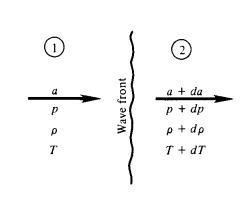
\includegraphics[width=0.3\linewidth]{screenshot001}
	\caption{}
	\label{fig:screenshot001}
\end{figure}

By applying a rectangular control volume around this pressure wave, we can apply our conservation equations. We are assuming that these properities are increasing by a small increment. This is why each variable is added by a infinitesimally small term.

Recalling the conservation of mass (continuity equation), $\dot{m} = constant$

\[\dot{m}_{left} = \dot{m}_{right}\]

Recalling he definition of density, $\rho = m/\bar{V}$ and rewriting $\bar{V} = uA$ (check the units)
\[\rho a \cancel{A}  = (\rho + d\rho)(a + da) \cancel{A}\]
Futher expanding gives,
\[\rho a   = (\rho a+ \rho da + a d\rho + da d\rho)\]

We say that $da d\rho$ is so small, we can assume it is zero. This is often referred to as "neglecting higher order terms (H.O.T)". The expression then becomes

\[\frac{da}{a} = -\frac{d \rho}{\rho}\]

For the momentum equation $P + \rho u^2 = constant$
\[P + \rho a^2  = P + dP +  (\rho + d\rho)(a + da)(a + da) \]

But we just said that $\rho a = (\rho + d\rho)(a + da)$


\[P + \rho a^2  = P + dP +  \rho a(a + da) \]
\[dP + \rho ada = a\]

Multiplying the second term by a and divide by a, this is essentially multiplying the second term by one.

\[dP + \rho a^2\frac{da}{a} = a\]

recalling the relation $\frac{da}{a} = -\frac{d \rho}{\rho}$

\[dp - a^2 d \rho = 0\]

                       \[a^2 = \frac{dp}{d\rho}\]

Since a sound wave is a very weak wave, when it travels through a medium, it only increases the pressure and density, etc. slightly. The effect of this is that friction  and heat transfer can be neglected. Since friction cannot be undone, we call this an irreversible process. Whenever there is no transfer of heat, it is called this adiabatic. Thus, the propagation of sound is an adiabatic, reversible process, otherwise called isentropic. Isentropic implies no increase in entropy, which is \textit{not} true in the presence of shock waves.

In the case of a thermally perfect gas, we can say $P = \rho R T$

For a callorically perfect gas we can say $pv^{\gamma} = constant$, where $v$ is volume per unit mass, or specific volume

Differentiating and recalling that $v = 1/\rho$

\[a = \sqrt{\frac{\gamma P}{\rho}} = \sqrt{\gamma R T}\]


\[dm = \left( \rho u\right)_2 - \left(\rho u\right)_1\]
\[D(mV) = \left(\rho u^2 + P \right)_2\]

For Steady flow,

\[\cancel{dm} = \left( \rho u\right)_2 - \left(\rho u\right)_1\]

\[ \left( \rho u\right)_1 = \left(\rho u\right)_2\]

Similarly, for the Momentum equation,

\[\left(\rho u^2 + P\right)_1 = \left(\rho u^2 + P\right)_2\]

Let us change the coordinate system motion for the traveling wave be independent of time, and thus corresponds to \textit{steady state} wave propagation. 
\[ u_1 = \bar{u} + a - \frac{1}{2} \partial u \]
\[ u_2 = \bar{u} + a + \frac{1}{2} \partial u \]


where, $\bar{u}$ is the average flow velocity and $a$ is the wave speed.


Substituting this back into the conservation of mass

\[\left(\rho u\right)_1 = \left(\rho u\right)_2 \]

\[ 
\left( \rho    - \frac{1}{2}\partial \rho \right) 
\left( \bar{u} - a - \frac{1}{2}\partial u\right) = 
\left( \rho    + \frac{1}{2}\partial \rho \right) 
\left( \bar{u} - a + \frac{1}{2}\partial u\right) 
\]

Further expanding

\[
\cancel{
	\rho \bar{u} - \rho a
} + 
\frac{1}{2} 
\left(
-\rho \partial u - \bar{u} - \bar{u} \partial \rho + a \partial \rho 
\right) +
\cancel{
	\frac{1}{4}\partial \rho \partial u 
}
= 
\cancel{
	\rho \bar{u} - \rho a
} + 
\frac{1}{2} 
\left(
\rho \partial u + \bar{u} - \bar{u} \partial \rho - a \partial \rho 
\right) +
\cancel{
	\frac{1}{4}\partial \rho \partial u 
}
\]
 
\[
  \frac{1}{2}\left( - \rho \partial u - \bar{u} \partial \rho + a \partial \rho\right) = 
  \frac{1}{2}\left(   \rho \partial u + \bar{u} \partial \rho - a \partial \rho\right)
\]

\[
\rho \partial u + u \partial \rho - a \partial \rho = 0 
\]

\[
\rho \partial u + \left( u - a\right)\partial \rho = 0
\]

Momentum Equation

\[
\left(\rho u^2 + P\right)_1 = 
\left(\rho u^2 + P\right)_2\]



\section{Appendix B: Isentropic Waves}

\[dU = dW + dQ\]

For adiabatic, reversible processes, the work done by a system with constant pressure and a change in volume is $-pdV$ and the change in heat energy is zero. Hence,

\[dU = -pdV\].

The change in enthalpy of such a system can be found by taking the derivative of its expression for a thermodynamic process 

\[H = U + pV\]

\[dH = dU + pdV + vdP\]

\[dH = -pdV + pdV + vdP\]

\[dH = vdP\]

The specific heats at constant pressure and constant volume 

\[\left(\frac{\partial U}{\partial T}\right)_v = C_v\]

\[\left(\frac{\partial H}{\partial T}\right)_p = C_p\]

\[\gamma = \frac{C_p}{C_v} = \frac{dH}{dU} = -\frac{VdP}{pdV} = -\frac{V}{dV}\frac{dP}{p}\]

Integrating both sides

\[\gamma \frac{dV}{V} = \frac{-dP}{P} \rightarrow \gamma \int \frac{1}{V} dV = - \int \frac{1}{P} dP\]

\[\gamma ln(V) + ln(P) = C\]

Using log rules

\[ln(V^\gamma) + ln(P) = C\]
 \[ln(pV^\gamma) = C \]
 \[pV^\gamma = e^C = C\]
 
 \[\frac{p}{\rho^\gamma}\]
 



\bibliography{References}
\bibliographystyle{unsrt}
\end{document}
